%%%%%%%%%%%%%%%%%%%%%%%%%%%%%%%%%%%%%%%%%%%%%%%%%%%%%%%%%%%%
% Manuscript started: 2008/10/12
% First completed draft: 2008/??/??, Vitamin D, Inc.
% Submission draft: 2008/??/??, Vitamin D, Inc.
%%%%%%%%%%%%%%%%%%%%%%%%%%%%%%%%%%%%%%%%%%%%%%%%%%%%%%%%%%%%

\documentclass[oneeqnum,onefignum,onetabnum,onethmnum]{siamltex}
\usepackage{graphics}
\usepackage{multirow}

% Macros for entire document

% Utility commands
\newcommand{\bc}{\begin{center}}
\newcommand{\ec}{\end{center}}
\newcommand{\beq}{\begin{equation}}
\newcommand{\eeq}{\end{equation}}
\newcommand{\bea}{\begin{eqnarray}}
\newcommand{\eea}{\end{eqnarray}}
\newcommand{\ba}{\begin{array}}
\newcommand{\ea}{\end{array}}

% Fancy equation environments
\newcommand{\Eq}[2][Eq.~]{{#1}(\ref{eq:#2})}                                    
\newcommand{\Eqs}[1]{Eqs.~(\ref{eq:#1})}                                        
\newcommand{\Fig}[2][Fig.~]{{#1}\ref{fig:#2}}                                   
\newcommand{\Figs}[1]{Figs.~\ref{fig:#1}}                                       
\newcommand{\Sec}[2][Sec.~]{{#1}\ref{sec:#2}}                                   
\newcommand{\Secs}[1]{Secs.~\ref{sec:#1}}      

% Common expressions
\def\eg{\emph{e.g., }}
\def\ie{\emph{i.e., }}
\def\etal{\emph{et al.}}
\def\etc{\emph{etc.}}

% Mathematical notation
\def\div{\ensuremath{\nabla \cdot}}
\def\divs{\ensuremath{\nabla_{s} \cdot}}
\def\grad{\ensuremath{\nabla}}
\def\grads{\ensuremath{\nabla_{s}}}
\def\lapl{\ensuremath{\nabla^2}}
\def\Real{\ensuremath{\mathrm{Re}}}
\newcommand{\tensor}[1]{\ensuremath{{\bf{#1}}}}

\newcommand{\ddx}[2]{\frac{\partial #1}{\partial #2}}
\newcommand{\DDx}[2]{\frac{D #1}{D #2}}
\newcommand{\sgn}[1]{\ensuremath{\mathrm{sgn}(#1)}}
\newcommand{\abs}[1]{\ensuremath{\left|#1\right|}}


% MATH MACROS
\def\sech{\mathrm{sech}}
\def\erfc{\mathrm{erfc}}

% PDE MACROS
\def\pt{\partial t}
\def\px{\partial x}
\def\py{\partial y}
\def\tu{\tilde{u}}

% NUMERICS MACROS
\def\dt{\Delta t}
\def\dx{\Delta x}
\def\dy{\Delta y}
\def\dy{\Delta y}
\def\dto{\dt_{opt}}


\title{High-Order Accurate Finite Difference Schemes \\
       for Variable-Coefficient PDEs via Optimal Time Step Selection}

\author{
Kevin T. Chu\footnotemark[2] \footnotemark[3]
and 
James V. Lambers\footnotemark[4]
}

\begin{document}
\bibliographystyle{unsrt}
\maketitle

\renewcommand{\thefootnote}{\fnsymbol{footnote}}
\footnotetext[2]{Vitamin D, Inc., Menlo Park, CA 94025} 

\renewcommand{\thefootnote}{\fnsymbol{footnote}}
\footnotetext[3]{Institute of High Performance Computing, A*STAR, Singapore, Singapore} 

\renewcommand{\thefootnote}{\fnsymbol{footnote}}
\footnotetext[4]{Department of Energy Resources Engineering, Stanford University, Stanford, CA 94305}

\renewcommand{\thefootnote}{\arabic{footnote}}


\begin{abstract}
place holder
\end{abstract}


\begin{keywords}
optimal time step, finite difference schemes, high-order accurate numerical 
methods, time dependent PDEs, variable-coefficient PDEs
\end{keywords}

\begin{AMS}
65-02, 65M06, 65M12, 65M20 ??
\end{AMS}

\pagestyle{myheadings}
\thispagestyle{plain}
\markboth{KEVIN T. CHU AND JAMES V. LAMBERS}
         {??}


\section*{Introduction}
Place holder...
\cite{zoppou1999, kreiss2002, guidotti2006}

Key points
\begin{itemize}
\item OTS applicable to problems with variable-coefficient equations by
      (1) optimally selecting the computational mesh or 
      (2) solving the equations on a transformed domain.  
      These two approaches are essentially the same.
\item Demonstration of OTS on discretization on a non-single step time 
      integration schemes.
\item Demonstration of boost in order of accuracy for variable-coefficient 
      wave equation. 
\item Demonstration of boost in order of accuracy for variable-coefficient 
      diffusion equation. 
\item Demonstration of boost in order of accuracy for 2D problem. Schrodinger
      equation?
\end{itemize}


\section{Optimal Time Step Selection for Variable-Coefficient PDEs}
Place holder...



\section{Wave Equation}
Second-order wave equation with source term:
\bea
    u_{tt} - c^2 u_{xx} = f.
    \label{eq:wave_eqn}
\eea
on the domain $-1 < x < 1$ subject to periodic boundary conditions and
initial conditions
\bea
  u(x,0)   &=& 2 \exp \left( -10 (\sin(0.5 \pi x))^2 \right) \nonumber \\
  u_t(x,0) &=& -0.5 \pi \sin(\pi x) + g(x)
\eea


\subsection{OTS Selection for Kriess-Petersson-Ystr\"om Discretization}
In~\cite{kreiss2002}, Kriess, Petersson, and Ystr\"om analyzed the following
direct discretization of the second-order wave equation without conversion 
to a first-order system of equations:
\bea
    \frac{u^{n+1}_i - 2 u^n_i + u^{n-1}_i}{\dt^2}
  = c^2 \left( \frac{u^{n}_{i+1} - 2 u^n_i + u^n_{i-1}}{\dx^2} \right)
  + f
  \label{eq:wave_eqn_KPY}
\eea
This scheme is second-order accurate in space and time and stable when 
$\dt < ??$.

To compute the optimal time step and correction terms for this scheme, we 
begin by deriving the evolution equation for the error, 
$e^n_i = u^n_i - \tu^n_i$, where $\tu^n_i \equiv \tu(i\dx, n\dt)$.  Employing
Taylor series expansions, it is straightforward to show that the true solution
satisfies:
\bea
  \frac{\tu^{n+1}_i - 2 \tu^n_i + \tu^{n-1}_i}{\dt^2}
    &-& \frac{\dt^2}{12} \tu_{tttt} + O(\dt^4)
  = \nonumber \\
  & & c^2 \left( \frac{\tu^{n}_{i+1} - 2 \tu^n_i + \tu^n_{i-1}}{\dx^2} 
             -\frac{\dx^2}{12} \tu_{xxxx} + O(\dx^4)
        \right)
  + f
\eea
Therefore, the error evolution equation is 
\bea
  \frac{e^{n+1}_i - 2 e^n_i + e^{n-1}_i}{\dt^2}
    &+& \frac{\dt^2}{12} \tu_{tttt} + O(\dt^4)
  = \nonumber \\
  & & c^2 \left( \frac{e^{n}_{i+1} - 2 e^n_i + e^n_{i-1}}{\dx^2} 
             +\frac{\dx^2}{12} \tu_{xxxx} + O(\dx^4)
        \right)
  \label{eq:wave_eqn_error_eqn}
\eea
Using the wave equation (\ref{eq:wave_eqn}) to express $\tu_{tttt}$ in terms
of spatial derivatives, we find that
\beq
  \tu_{tttt} = c^4 \tu_{xxxx} + c^2 f_{xx} + f_{tt}
\eeq
Substituting this result into (\ref{eq:wave_eqn_error_eqn}), we find that
\bea
  \frac{e^{n+1}_i - 2 e^n_i + e^{n-1}_i}{\dt^2}
    &+& \frac{\dt^2}{12} \left(c^4\tu_{xxxx} + c^2 f_{xx} + f_{tt} \right) 
    + O(\dt^4)
  = \nonumber \\
  & & c^2 \left( \frac{e^{n}_{i+1} - 2 e^n_i + e^n_{i-1}}{\dx^2} 
             +\frac{\dx^2}{12} \tu_{xxxx} + O(\dx^4)
        \right)
\eea
Thus, we see that we can eliminate the leading-order term in the discretization
error by choosing $\dt = \dx/c$ and adding the correction term 
\beq
  \frac{\dt^2}{12} \left(c^2 f_{xx} + f_{tt} \right) 
\eeq
to the right-hand side of (\ref{eq:wave_eqn_KPY}).  

With this choice of time step and the correction term, the local truncation
error is $O(\dt^6) + O(\dx^4 \dt^2)$.  Using the heuristic for single-step 
calculations leads to the conclusion that the global error should be 
approximately $1/\dt^2$ times the local error, which leads to a global error
of $O(\dx^4) = O(\dt^4)$.  
Figures~\ref{fig:wave_eqn_no_src_error} and~\ref{fig:wave_eqn_src_error} 
demonstrate that the expected accuracy is achieved. 

Note that to get higher-order accuracy, we also need to use a fifth-order
accurate first step for the scheme.  For the wave equation, this is 
straightforward to achieve by using a fifth-order Taylor series expansion
in time to obtain $u^1_i$.  The reason that the first time step needs to be 
fifth-order accurate can be seen by observing that the solution of the 
difference equation for the normal modes (von Neumann analysis):
\bea
  \frac{e^{n+1} - 2 e^{n} + e^{n-1}}{\dt^2} = \dt^2 \lambda e^{n}
  \label{eq:error_eqn_normal_mode}
\eea
is~\cite{carrier_pearson_book}
\bea
  e^n = e^1 \frac{\kappa_+^n - \kappa_-^n}{\kappa_+ - \kappa_-} 
      + e^0 \kappa_+ \kappa_- 
        \frac{\kappa_+^{n-1} - \kappa_-^{n-1}}{\kappa_+ - \kappa_-} 
  \label{eq:error_eqn_normal_mode_soln}
\eea
where $\kappa_\pm$, the roots of the characteristic equation for 
(\ref{eq:error_eqn_normal_mode}), are given by~\cite{kreiss2002}
\beq
  \kappa_\pm = 1 + \frac{1}{2} \lambda \dt^2 
             \pm \dt \sqrt{\lambda + \frac{\lambda^2 \dt^2}{4}}.
\eeq
From the solution to the error equation for the normal modes 
(\ref{eq:error_eqn_normal_mode_soln}), we see that the solution loses
one temporal order of accuracy compared to the initial conditions because
the denominator of both terms is $O(\dt)$.
In other words, the initial errors $e^0$ and $e^1$ must be $O(\dt^5)$ in 
order to for the solution to be $O(\dt^4)$.  


\begin{figure}[thb]
\begin{center}
\scalebox{0.35}{\includegraphics{figures/wave_eqn_1d_no_src_error_vs_N}}
\caption{$L^\infty$ error as a function of number of grid points for the
KPY discretization of the second-order wave equation without source term.
}
\label{fig:wave_eqn_no_src_error}
\end{center}
\end{figure}

\begin{figure}[thb]
\begin{center}
\scalebox{0.35}{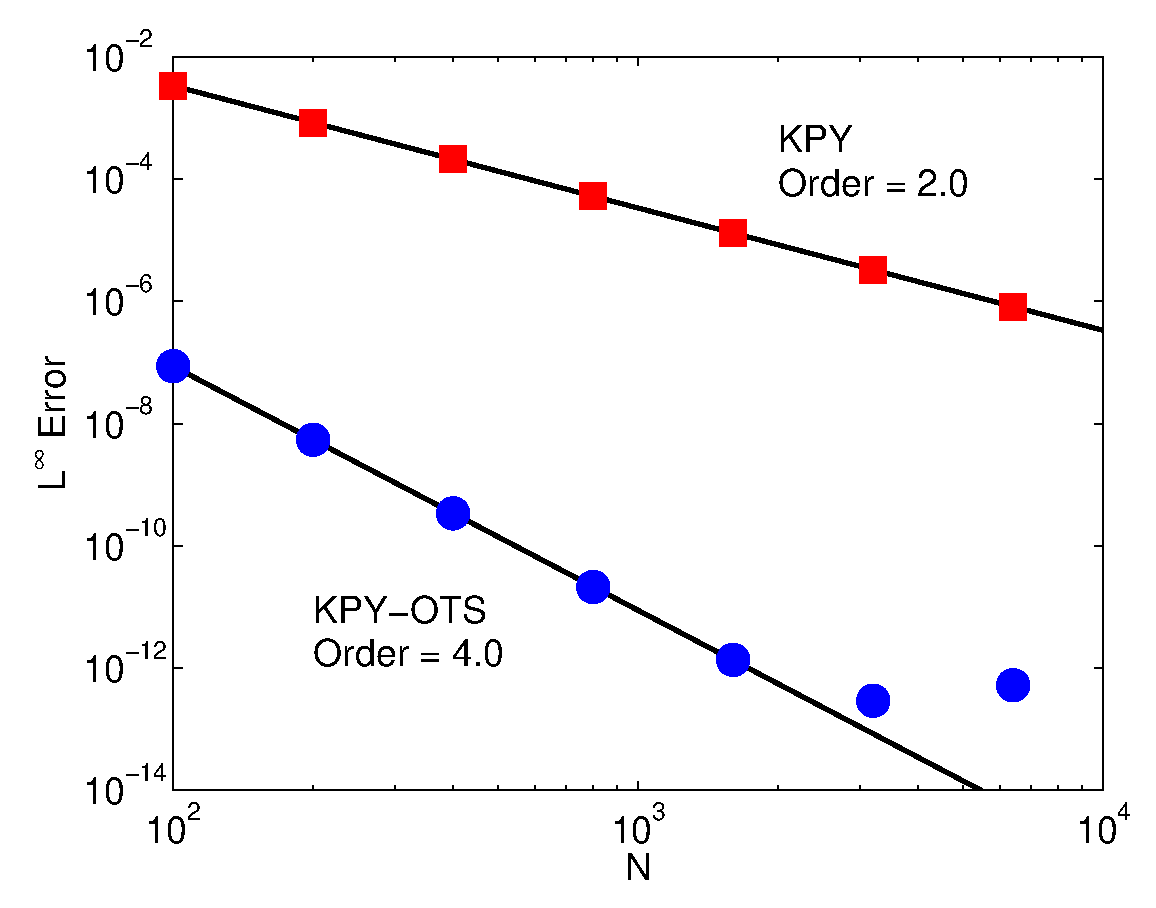
\includegraphics{figures/wave_eqn_1d_src_error_vs_N}}
\caption{$L^\infty$ error as a function of number of grid points for the
KPY discretization of the second-order wave equation with source term.
}
\label{fig:wave_eqn_src_error}
\end{center}
\end{figure}



\subsection{OTS Selection for Variable Coefficient Wave Equation}
We consider the variable-coefficient second-order wave equation:
\beq
    u_{tt} - c(x)^2 u_{xx} = f,
    \label{eq:var_coef_wave_eqn}
\eeq
on the domain $-1 < x < 1$.

The formulation of optimal time step selection presented in~\cite{chu2009}
is restricted to problems which are constant coefficient in the leading-order 
temporal and spatial derivatives.  To extend apply the technique to the
variable-coefficient wave equation, we can take one of two approaches:
(1) transformation of the domain so that the leading-order equations are 
constant coefficient or (2) use of an optimal computational grid with
variable grid spacing when solving the equation on the original domain.
In fact, these two approaches are closely related because the optimal 
computational grid is the mapping of a uniform grid in the transformed domain
onto the original domain.

Following~\cite{guidotti_2006}, we use the following simple change of variables
to transform (\ref{eq:var_coef_wave_eqn}) into a constant coefficient 
wave equation:
\beq
  y = \Phi(x) = \cbar \int_{-1}^x \frac{1}{c(\xi)} d\xi,
\eeq
where 
\beq
  \cbar = \left( \int_{-1}^1 \frac{1}{c(\xi)} d\xi \right)^{-1}.
\eeq
On the transformed domain, (\ref{eq:var_coef_wave_eqn}) becomes
\beq
  u_{tt} = 4\cbar^2 u_{yy} - 2 \cbar c' u_y + f,
\eeq
where $c' = dc/dx$.


\subsection{OTS on Transformed Domain}
If we use second-order central differences for both the Laplacian and 
gradient terms, the optimal time step remains the same as for the constant
coefficient wave equation $\dt = \dx/2 \cbar$.  The correction term is also
straightforward (but tedious) to calculate:
\bea
  \frac{\dt^2}{12} 
  \left(
    \begin{array}{l}
        -16 \cbar^3 (c')_y u_{yy}
        -8 \cbar^3 (c')_{yy} u_{y}
        +4 \cbar^2 (c')^2 u_{yy} 
        \\
        +\ 4 \cbar^2 c' (c')_y u_{y}
        +4 \cbar^2 f_{yy}
        -2 \cbar c' f_y
        + f_{tt}
    \end{array}
  \right)
\eea
With the optimal time step and this correction term, we obtain a third-order
accurate scheme for the variable-coefficient wave equation.  
Figure~\ref{fig:var_coef_wave_eqn_src_error} shows the results.

\begin{figure}[thb]
\begin{center}
\scalebox{0.35}{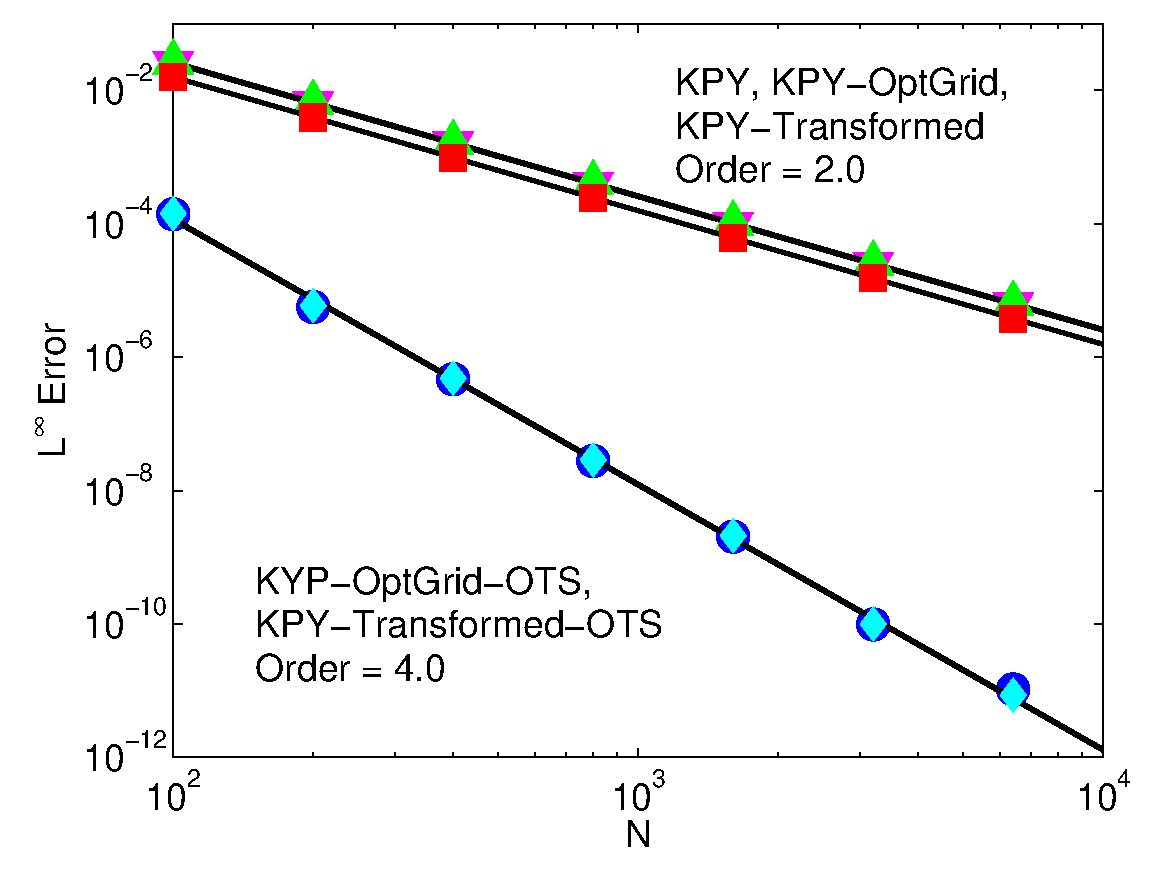
\includegraphics{figures/var_coef_wave_eqn_1d_error_vs_N}}
\caption{$L^\infty$ error as a function of number of grid points for the
KPY discretization of the variable-coefficient second-order wave equation 
with source term.
}
\label{fig:var_coef_wave_eqn_src_error}
\end{center}
\end{figure}

\subsection{OTS with Optimal Mesh}
While applying OTS to the equation on the transformed domain yields a
boost in order of accuracy, the lower-order spatial derivative and the
correction term are tedious to deal with.  A convenient alternative is to 
work on the original domain but optimally choose the mesh so that use of
an optimal time step still leads to fortuitous cancellation of the 
leading-order error.  

We calculate the location of the grid points in the optimal mesh by mapping
a uniform mesh in the $y$-domain back to the $x$-domain.  The finite 
difference stencil for the Laplacian on this mesh is natural generalization 
of Laplaacian to irregularly spaced grid points:
\bea
  (u_{xx})_i &\approx&
    \frac{1}{(x_{i+1}+x_i)/2 - (x_i+x_{i-1})/2}
    \left( \frac{u_{i+1}-u_i}{x_{i+1} - x_i}
         - \frac{u_{i}-u_{i-1}}{x_{i} - x_{i-1}}
    \right)
  \nonumber \\
  &=&
    \frac{2}{x_{i+1}-x_{i-1}}
    \left( \frac{u_{i+1}-u_i}{x_{i+1} - x_i}
         - \frac{u_{i}-u_{i-1}}{x_{i} - x_{i-1}}
    \right)
\eea

Using our analysis of the problem in the transformed domain, we find that the
optimal time step for the scheme on the variable mesh is given by
$\dt_{opt} = \dy/2\cbar$.  The correction term can be derived by first
computing $u_{tttt}$ on the original domain
\bea
  u_{tttt} = 
    c^4 u_{xxxx}
  + c^2 \left( (c^2)_xx u_{xx} + 2 (c^2)_x u_{xxx} + f_{xx} \right)
  + f_{tt}
\eea
Because the odd derivatives do not show up in the correction term on
the transformed domain (they cancelled themselves out), the odd derivative
is not part of the correction term for the scheme on the variable mesh.  
Thus, the correction term is
\beq
  \frac{\dt^2}{12} \left[ c^2 (c^2)_xx u_{xx} + c^2 f_{xx} + f_{tt} \right]
\eeq

Using the optimal time step and this correction term yields a third-order 
accurate scheme for the variable-coefficient wave equation.  The error on
the variable mesh is almost identical to the error obtained when solving
the equation on the transformed domain (see 
Figure~\ref{fig:var_coef_wave_eqn_src_error}).

*** KTC: 
I haven't thought of a nice elegant way to derive the optimal time
step and correction term yet... 
***


\section{Diffusion Equation}
Not done yet...


% ACKNOWLEDGMENTS
\section*{Acknowledgments}
K.T. Chu gratefully acknowledges the support of Vitamin D, Inc.
and the Institute for High-Performance Computing (IHPC) in Singapore. 
The authors would like to thank ??
for helpful suggestions on the manuscript.  

\bibliography{OTSPDE-VarCoefs}

\end{document}
